\section{Modes}

\subsection{Diatonic modes}

So far we have seen the major and minor scales. Both the diatonic and pentatonic versions. And all starting from the 6th string. This will allow you to improvise a nice melody over a song.

But, did you realize that the notes in the (diatonic) C major scale (\autoref{tab:guitar_c_major_scale}) and the A minor scale (\autoref{tab:guitar_a_minor_scale}) are the same? That is because the \textbf{relative minor} of a major scale starts at the 6th index of the major scale. In \autoref{tab:guitar_mode_intervals} you see that by starting on the 6th note, you get the intervals of the natural minor scale (also called \textnormal{A}eolian).

So d\textnormal{o}es that mean that you can improvise with the notes of A minor scale over a song in C major. YES!. After all, they are the same notes.

D\textnormal{o}es that mean that C major and A minor are identical. \textbf{No}. That also means that you can only say that a song is in C major, A minor, E phrygian, etc. by looking at the \mbox{\textbf{tonal center}} (the tone that is most prominent) of the musical context (chord progression). 

\underline{A mnemonic for the mode name order: \textbf{I} \textbf{D}on't \textbf{P}articularly \textbf{L}ike \textbf{M}odes \textbf{A} \textbf{Lo}t.}

\begin{table}[h]
	\centering
	\begin{tabular}{*{30}{c}}
		Ionian (major) & & \multicolumn{2}{P{4mm}}{\large{W}} & \multicolumn{2}{P{4mm}}{\large{W}} & \multicolumn{2}{P{4mm}}{\large{H}} & \multicolumn{2}{P{4mm}}{\large{W}} & \multicolumn{2}{P{4mm}}{\large{W}} & \multicolumn{2}{P{4mm}}{\large{W}} & \multicolumn{2}{P{4mm}}{\large{H}} & \\
		\textit{Chords} & \multicolumn{2}{P{4mm}}{\RomanNumeralCaps{1}} & \multicolumn{2}{P{4mm}}{\RomanNumeral{2}} & \multicolumn{2}{P{4mm}}{\RomanNumeral{3}} & \multicolumn{2}{P{4mm}}{\RomanNumeralCaps{4}} & \multicolumn{2}{P{4mm}}{\RomanNumeralCaps{5}} & \multicolumn{2}{P{4mm}}{\RomanNumeral{6}} & \multicolumn{2}{P{4mm}}{\RomanNumeral{7}\textsuperscript{o}} & \\
		\textit{Intervals} & \multicolumn{2}{P{4mm}}{1} & \multicolumn{2}{P{4mm}}{2} & \multicolumn{2}{P{4mm}}{3} & \multicolumn{2}{P{4mm}}{4} & \multicolumn{2}{P{4mm}}{5} & \multicolumn{2}{P{4mm}}{6} & \multicolumn{2}{P{4mm}}{7} & \\
		\hline \\
		Dorian & \multicolumn{3}{P{4mm}}{} & \multicolumn{2}{P{4mm}}{\large{W}} & \multicolumn{2}{P{4mm}}{\large{H}} & \multicolumn{2}{P{4mm}}{\large{W}} & \multicolumn{2}{P{4mm}}{\large{W}} & \multicolumn{2}{P{4mm}}{\large{W}} & \multicolumn{2}{P{4mm}}{\large{H}} & \multicolumn{2}{P{4mm}}{\large{W}} & \\
		& \multicolumn{2}{P{4mm}}{} & \multicolumn{2}{P{4mm}}{\RomanNumeral{1}} & \multicolumn{2}{P{4mm}}{\RomanNumeral{2}} & \multicolumn{2}{P{4mm}}{\RomanNumeralCaps{3}} & \multicolumn{2}{P{4mm}}{\RomanNumeralCaps{4}} & \multicolumn{2}{P{4mm}}{\RomanNumeral{5}} & \multicolumn{2}{P{4mm}}{\RomanNumeral{6}\textsuperscript{o}} & \multicolumn{2}{P{4mm}}{\RomanNumeralCaps{7}} & \\
		& \multicolumn{2}{P{4mm}}{} &  \multicolumn{2}{P{4mm}}{1} & \multicolumn{2}{P{4mm}}{2} & \multicolumn{2}{P{4mm}}{3\flat} & \multicolumn{2}{P{4mm}}{4} & \multicolumn{2}{P{4mm}}{5} & \multicolumn{2}{P{4mm}}{6} & \multicolumn{2}{P{4mm}}{7\flat} & \\
		\hline \\
		Phrygian & \multicolumn{5}{P{4mm}}{} & \multicolumn{2}{P{4mm}}{\large{H}} & \multicolumn{2}{P{4mm}}{\large{W}} & \multicolumn{2}{P{4mm}}{\large{W}} & \multicolumn{2}{P{4mm}}{\large{W}} & \multicolumn{2}{P{4mm}}{\large{H}} & \multicolumn{2}{P{4mm}}{\large{W}} & \multicolumn{2}{P{4mm}}{\large{W}} & \\
		& \multicolumn{4}{P{4mm}}{} & \multicolumn{2}{P{4mm}}{\RomanNumeral{1}} & \multicolumn{2}{P{4mm}}{\RomanNumeralCaps{2}} & \multicolumn{2}{P{4mm}}{\RomanNumeralCaps{3}} & \multicolumn{2}{P{4mm}}{\RomanNumeral{4}} & \multicolumn{2}{P{4mm}}{\RomanNumeral{5}\textsuperscript{o}} & \multicolumn{2}{P{4mm}}{\RomanNumeralCaps{6}} & \multicolumn{2}{P{4mm}}{\RomanNumeral{7}} & \\
		& \multicolumn{4}{P{4mm}}{} &  \multicolumn{2}{P{4mm}}{1} & \multicolumn{2}{P{4mm}}{2\flat} & \multicolumn{2}{P{4mm}}{3\flat} & \multicolumn{2}{P{4mm}}{4} & \multicolumn{2}{P{4mm}}{5} & \multicolumn{2}{P{4mm}}{6\flat} & \multicolumn{2}{P{4mm}}{7\flat} & \\
		\hline \\
		Lydian & \multicolumn{7}{P{4mm}}{} & \multicolumn{2}{P{4mm}}{\large{W}} & \multicolumn{2}{P{4mm}}{\large{W}} & \multicolumn{2}{P{4mm}}{\large{W}} & \multicolumn{2}{P{4mm}}{\large{H}} & \multicolumn{2}{P{4mm}}{\large{W}} & \multicolumn{2}{P{4mm}}{\large{W}} & \multicolumn{2}{P{4mm}}{\large{H}} & \\
		& \multicolumn{6}{P{4mm}}{} & \multicolumn{2}{P{4mm}}{\RomanNumeralCaps{1}} & \multicolumn{2}{P{4mm}}{\RomanNumeralCaps{2}} & \multicolumn{2}{P{4mm}}{\RomanNumeral{3}} & \multicolumn{2}{P{4mm}}{\RomanNumeral{4}\textsuperscript{o}} & \multicolumn{2}{P{4mm}}{\RomanNumeralCaps{5}} & \multicolumn{2}{P{4mm}}{\RomanNumeral{6}} & \multicolumn{2}{P{4mm}}{\RomanNumeral{7}} & \\
		& \multicolumn{6}{P{4mm}}{} &  \multicolumn{2}{P{4mm}}{1} & \multicolumn{2}{P{4mm}}{2} & \multicolumn{2}{P{4mm}}{3} & \multicolumn{2}{P{4mm}}{4\sharp} & \multicolumn{2}{P{4mm}}{5} & \multicolumn{2}{P{4mm}}{6} & \multicolumn{2}{P{4mm}}{7} & \\
		\hline \\
		Mixolydian & \multicolumn{9}{P{4mm}}{} & \multicolumn{2}{P{4mm}}{\large{W}} & \multicolumn{2}{P{4mm}}{\large{W}} & \multicolumn{2}{P{4mm}}{\large{H}} & \multicolumn{2}{P{4mm}}{\large{W}} & \multicolumn{2}{P{4mm}}{\large{W}} & \multicolumn{2}{P{4mm}}{\large{H}} & \multicolumn{2}{P{4mm}}{\large{W}} & \\
		& \multicolumn{8}{P{4mm}}{} & \multicolumn{2}{P{4mm}}{\RomanNumeralCaps{1}} & \multicolumn{2}{P{4mm}}{\RomanNumeral{2}} & \multicolumn{2}{P{4mm}}{\RomanNumeral{3}\textsuperscript{o}} & \multicolumn{2}{P{4mm}}{\RomanNumeralCaps{4}} & \multicolumn{2}{P{4mm}}{\RomanNumeral{5}} & \multicolumn{2}{P{4mm}}{\RomanNumeral{6}} & \multicolumn{2}{P{4mm}}{\RomanNumeralCaps{7}} & \\
		& \multicolumn{8}{P{4mm}}{} &  \multicolumn{2}{P{4mm}}{1} & \multicolumn{2}{P{4mm}}{2} & \multicolumn{2}{P{4mm}}{3} & \multicolumn{2}{P{4mm}}{4} & \multicolumn{2}{P{4mm}}{5} & \multicolumn{2}{P{4mm}}{6} & \multicolumn{2}{P{4mm}}{7\flat} & \\
		\hline \\
		\textnormal{A}eolian (natural minor) & \multicolumn{11}{P{4mm}}{} & \multicolumn{2}{P{4mm}}{\large{W}} & \multicolumn{2}{P{4mm}}{\large{H}} & \multicolumn{2}{P{4mm}}{\large{W}} & \multicolumn{2}{P{4mm}}{\large{W}} & \multicolumn{2}{P{4mm}}{\large{H}} & \multicolumn{2}{P{4mm}}{\large{W}} & \multicolumn{2}{P{4mm}}{\large{W}} & \\
		& \multicolumn{10}{P{4mm}}{} & \multicolumn{2}{P{4mm}}{\RomanNumeral{1}} & \multicolumn{2}{P{4mm}}{\RomanNumeral{2}\textsuperscript{o}} & \multicolumn{2}{P{4mm}}{\RomanNumeralCaps{3}} & \multicolumn{2}{P{4mm}}{\RomanNumeral{4}} & \multicolumn{2}{P{4mm}}{\RomanNumeral{5}} & \multicolumn{2}{P{4mm}}{\RomanNumeralCaps{6}} & \multicolumn{2}{P{4mm}}{\RomanNumeralCaps{7}} & \\
		& \multicolumn{10}{P{4mm}}{} &  \multicolumn{2}{P{4mm}}{1} & \multicolumn{2}{P{4mm}}{2} & \multicolumn{2}{P{4mm}}{3\flat} & \multicolumn{2}{P{4mm}}{4} & \multicolumn{2}{P{4mm}}{5} & \multicolumn{2}{P{4mm}}{6\flat} & \multicolumn{2}{P{4mm}}{7\flat} & \\
		\hline \\
		Locrian & \multicolumn{13}{P{4mm}}{} & \multicolumn{2}{P{4mm}}{\large{H}} & \multicolumn{2}{P{4mm}}{\large{W}} & \multicolumn{2}{P{4mm}}{\large{W}} & \multicolumn{2}{P{4mm}}{\large{H}} & \multicolumn{2}{P{4mm}}{\large{W}} & \multicolumn{2}{P{4mm}}{\large{W}} & \multicolumn{2}{P{4mm}}{\large{W}} & \\
		& \multicolumn{12}{P{4mm}}{} & \multicolumn{2}{P{4mm}}{\RomanNumeral{1}\textsuperscript{o}} & \multicolumn{2}{P{4mm}}{\RomanNumeralCaps{2}} & \multicolumn{2}{P{4mm}}{\RomanNumeral{3}} & \multicolumn{2}{P{4mm}}{\RomanNumeral{4}} & \multicolumn{2}{P{4mm}}{\RomanNumeralCaps{5}} & \multicolumn{2}{P{4mm}}{\RomanNumeral{6}} & \multicolumn{2}{P{4mm}}{\RomanNumeral{7}} & \\
		& \multicolumn{12}{P{4mm}}{} &  \multicolumn{2}{P{4mm}}{1} & \multicolumn{2}{P{4mm}}{2\flat} & \multicolumn{2}{P{4mm}}{3\flat} & \multicolumn{2}{P{4mm}}{4} & \multicolumn{2}{P{4mm}}{5\flat} & \multicolumn{2}{P{4mm}}{6\flat} & \multicolumn{2}{P{4mm}}{7\flat} & \\
	\end{tabular}
	\caption{Mode intervals}
	\label{tab:guitar_mode_intervals}
\end{table}

\newpage

\subsubsection{Using modes to give a different feeling}

So far we have looked at modes as being a variant of the major scale. Meaning that if a song is in C major, that you can play notes from all the different modes that are derived from C major (D dorian, E phrygian, etc.). Note that this assumes that the tonal center, the note that the songs always wants to come back to, is C. And by playing notes and chords from the C major scale, it gets the major feeling.

To get the feeling of a different mode, you most often want to start on the chords of your mode (so the D minor chord for D dorian), and then play chords that emphasize the characteristic notes in the mode.

What are the characteristic notes of the mode? For that we first have to determine if a mode if a major or minor chord. Things means looking at the 3rd index to see if it is a major or minor 3rd (3 or 3$\flat$). Next you compare the mode intervals with either the major or minor intervals and see which are different. This is shown in \autoref{tab:guitar_mode_characteristic_notes}.

\begin{table}[h]
	\centering
	\begin{tabular}{*{8}{c}}
		\textbf{Ionian (major)} & 1 & 2 & 3 & 4 & 5 & 6 & 7 \\
		Lydian (\textit{major}) & 1 & 2 & 3 & \ScaleCellFill 4$\sharp$ & 5 & 6 & 7 \\
		Mixolydian (\textit{major}) & 1 & 2 & 3 & 4 & 5 & 6 & \ScaleCellFill 7$\flat$ \\
		\\
		\textbf{\textnormal{A}eolian (natural minor)} & 1 & 2 & 3$\flat$ & 4 & 5 & 6$\flat$ & 7$\flat$ \\
		Dorian (\textit{minor}) & 1 & 2 & 3$\flat$ & 4 & 5 & \ScaleCellFill 6 & 7$\flat$ \\
		Phrygian (\textit{minor}) & 1 & \ScaleCellFill 2$\flat$ & 3$\flat$ & 4 & 5 & 6$\flat$ & 7$\flat$ \\
		Locrian (\textit{diminished}) & 1 & \ScaleCellFill 2$\flat$ & 3$\flat$ & 4 & \ScaleCellFill 5$\flat$ & 6$\flat$ & 7$\flat$ \\
	\end{tabular}
	\caption{Mode characteristic notes}
	\label{tab:guitar_mode_characteristic_notes}
\end{table}

The next step is to see which chords in the mode that you want to play have the characteristic note. This is important because we really want to emphasis the tonal center of the mode to give the right 'feel'. In \autoref{sec:building_chords_with_diatonic_scale} you learned how to build chords from the diatonic scales. The chords in \autoref{tab:guitar_mode_intervals} are created the same way. With this knowledge the table \autoref{tab:guitar_mode_characteristic_chords} can be created that shows which chords of the mode are characteristic for the mode. This table is limited to the 3-note chords and (maj)7th chords. But you can off course alter a chord to become, for example, sus2 chords which would add the characteristic note in the chord. 

\begin{table}[h]
	\centering
	\begin{tabular}{*{5}{c}}
		\textbf{Ionian (major)} &  \\
		Lydian (\textit{major}) & \RomanNumeralCaps{2} & \RomanNumeral{4}\textsuperscript{o} & \RomanNumeralCaps{5}maj7 & \RomanNumeral{7}  \\
		Mixolydian (\textit{major}) & \RomanNumeralCaps{1}7 & \RomanNumeral{3}\textsuperscript{o} & \RomanNumeral{5} & \RomanNumeralCaps{7} \\
		\\
		\textbf{\textnormal{A}eolian (natural minor)} & \\
		Dorian (\textit{minor}) &  \RomanNumeral{2} & \RomanNumeralCaps{4} & \RomanNumeral{6}\textsuperscript{o} & \RomanNumeralCaps{7}maj7 \\
		Phrygian (\textit{minor}) &  \RomanNumeralCaps{2} & \RomanNumeralCaps{3}7 & \RomanNumeral{4} & \RomanNumeralCaps{6} \\
		Locrian (\textit{diminished}) & all \\
	\end{tabular}
	\caption{Mode characteristic chords}
	\label{tab:guitar_mode_characteristic_chords}
\end{table}

Now when you create a chord progression for a mode, it would be good to use at least one chord listed in \autoref{tab:guitar_mode_characteristic_chords} besides having the first chord of the mode.

\newpage

\subsubsection{Using modes-shapes to open up the fretboard}

\autoref{fig:guitar_diatonic_modes_on_guitar} shows the different \textbf{mode-shapes}. In this case we start with F$\sharp$ Ionian (major) scale. But remember that these can be shifted up or down to be in a different key.

The gray frets with number on the 6th string show the F$\sharp$ major scale on the 6th string. This is used to show the connection between the starting position of the different modes with the major scale intervals. Because we are looking from the major scale's perspective, the numbers in the frets of a shape also correspond to the intervals in the major scale.

Just as before, the different colors indicate different octaves in the shape. Meaning that each shape covers 2 and a bit octaves.

\infobox
{
	\begin{itemize}
		\item The mode names in \autoref{fig:guitar_diatonic_modes_on_guitar} correspond to the shape in this case.
		\item The relative position of these shapes simply cover the whole fretboard with notes of a certain scale/mode.
		\item All shapes shown in \autoref{fig:guitar_diatonic_modes_on_guitar} are relative to the F$\sharp$ major scale (ionian mode). If they would be relative to the G$\sharp$ dorian mode then the shapes would be the same, but the numbers would be different. If they would be relative to G dorian mode, then all the shapes would move one fret down (to the left). 
	\end{itemize}
}

\newpage

\begin{figure}[h]
	\centering
	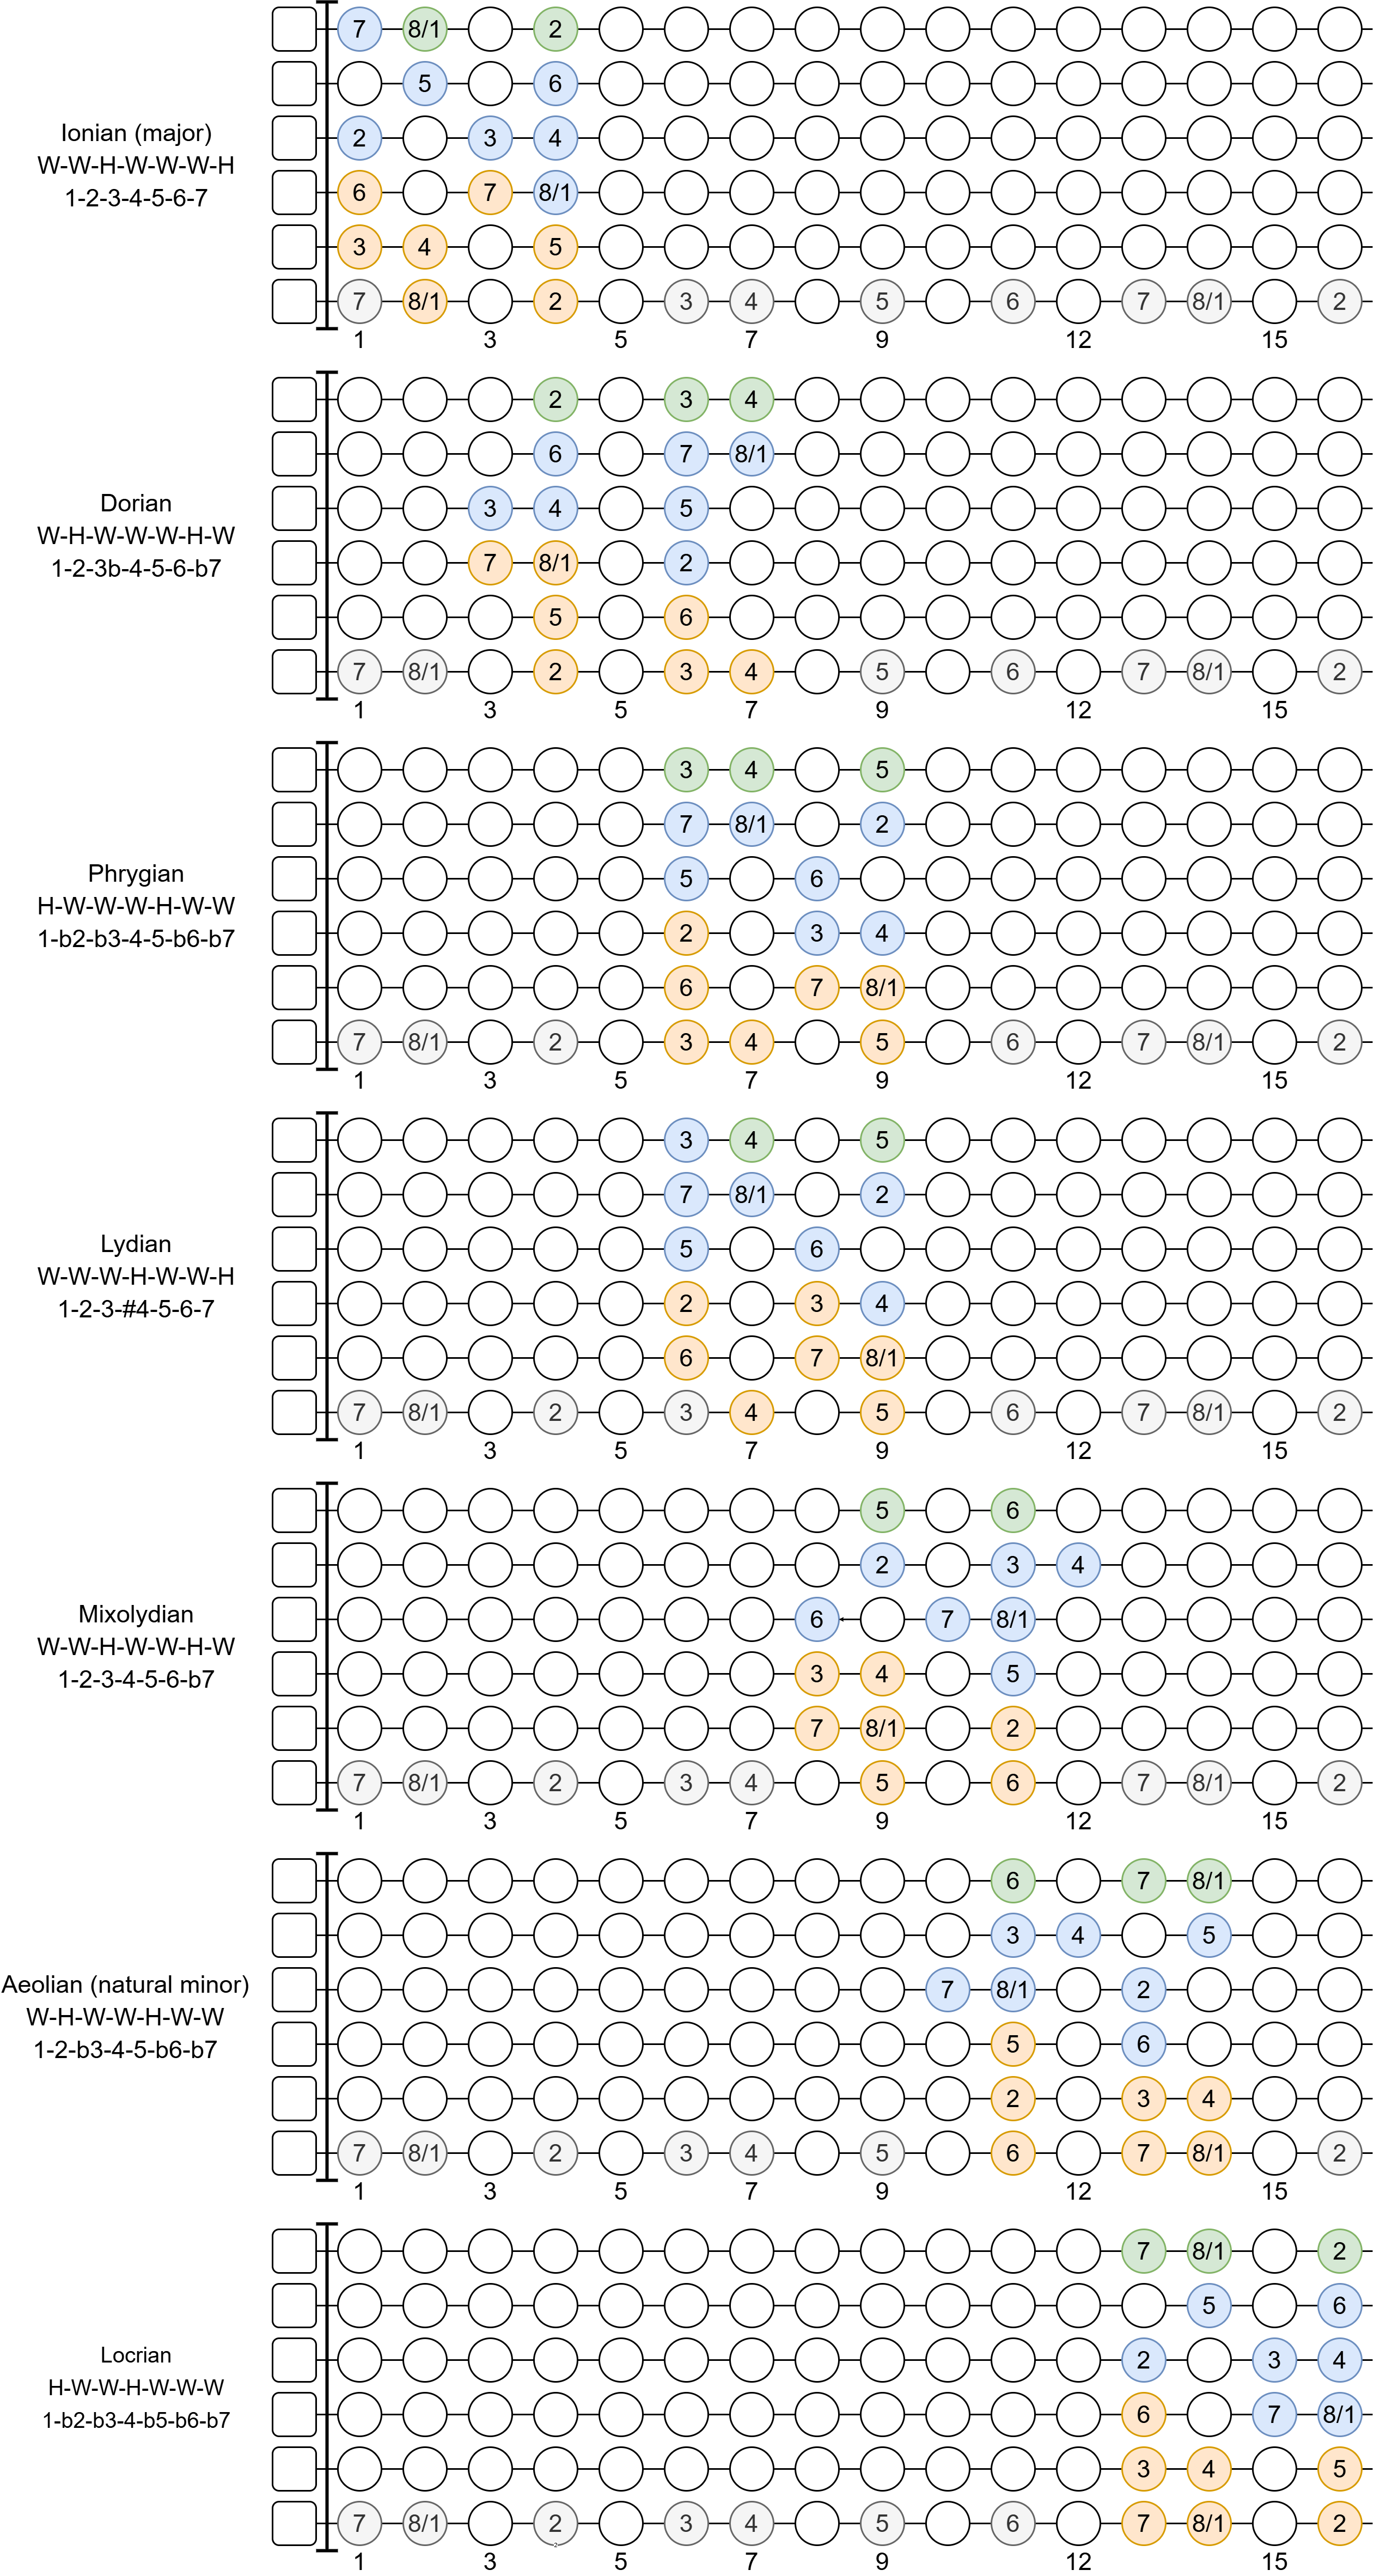
\includegraphics[width=0.9\textwidth]{../../Images/guitar_mode_all.png}
	\caption{Diatonic modes on the guitar}
	\label{fig:guitar_diatonic_modes_on_guitar}
\end{figure}

\clearpage

\subsection{Pentatonic modes}
TODO

\section{CAGED}
TODO